\selectlanguage{italian}

\section{Proprietà generali}

La forma tipica di una reazione nucleare è la seguente:
\begin{equation*}
	\mathrm{a} + \mathrm{X} \rightarrow \mathrm{Y} + \mathrm{b}
\end{equation*}
dove $ \mathrm{X} $ e $ \mathrm{Y} $ sono nuclidi target-like, $ \mathrm{a} $ e $ \mathrm{b} $ projectile-like. Una scrittura alternativa è: $ \mathrm{X} \left( \mathrm{a},\mathrm{b} \right) \mathrm{Y} $.\\
In linea generale, le reazioni nucleari soddisfano alcune leggi di conservazione, sebbene alcune di esse non in maniera sempre esatta: energia totale, momento lineare totale, momento angolare totale, carica elettrica totale, parità, numero atomico. In base all'energia per nucleone possono presentarsi comportamenti aggiuntivi:
\begin{enumerate}
	\item low-energy ($ E \lesssim 10\mev $ per nucleone): non ci sono processi legati all'interazione forte, dunque si conservano anche il numero di protoni e quello di neutroni;
	\item medium-energy ($ 100\mev \lesssim E \lesssim 1\gev $ per nucleone): subentrano processi di meson production, dunque protoni e neutroni possono trasformarsi gli uni negli altri;
	\item high-energy ($ E \gtrsim 10\gev $ per nucleone); possono essere prodotte molte particelle esotiche, arrivando a riarrangiare anche i quarks nei nucleoni.
\end{enumerate}
Inoltre, dato che affinché avvenga la reazione si deve superare la barriera coulombiana nei nuclei, è necessario che la reazione abbia un certo $ Q $-value. Dalla conservazione dell'energia totale si ha:
\begin{equation*}
	M_{\mathrm{a}} c^2 + T_{\mathrm{a}} + M_{\mathrm{X}} c^2 T_{\mathrm{X}} = M_{\mathrm{Y}} c^2 + T_{\mathrm{Y}} + M_{\mathrm{b}} c^2 + T_{\mathrm{b}}
	\quad \Rightarrow \quad
	Q = M_{\mathrm{a}} c^2 + M_{\mathrm{X}} c^2 - \left( M_{\mathrm{Y}} c^2 + M_{\mathrm{b}} c^2 \right)
\end{equation*}
Se $ Q > 0 $ si parla di \textit{reazione esoergonica} (o esotermica), nella quale parte della massa nucleare o della binding energy viene liberata sotto forma di energia cinetica, mentre se $ Q < 0 $ di \textit{reazione endoergonica} (o endotermica), nella quale parte dell'energia cinetica è convertita in massa nucleare o binding energy. Nel caso in cui $ Q = 0 $ si parla di \textit{collisione elastica}.\\
Una reazione è sempre possibile se $ Q \ge 0 $, mentre se $ Q < 0 $ è necessario che $ T_{\mathrm{a}} $ superi una certa threshold energy:
\begin{equation}
	T_{\text{th}} = -Q \frac{M_{\mathrm{Y}} + M_{\mathrm{b}}}{M_{\mathrm{Y}} + M_{\mathrm{b}} - M_{\mathrm{a}}}
	\label{eq:6.1}
\end{equation}
Dalla conservazione dell'impulso, invece, considerando il laboratory frame in cui il target $ \mathrm{X} $ è a riposo e definendo $ \theta $ e $ \xi $ gli angoli tra i momenti di $ \mathrm{Y} $ e $ \mathrm{b} $ e quello di $ \mathrm{a} $, si ha:
\begin{equation*}
	\begin{cases}
		p_{\mathrm{a}} = p_{\mathrm{b}} \cos \theta + p_{\mathrm{Y}} \cos \xi \\
		0 = p_{\mathrm{b}} \sin \theta - p_{\mathrm{Y}} \sin \xi
	\end{cases}
\end{equation*}
Si hanno tre equazioni in quattro incognite ($ T_{\mathrm{b}}, T_{\mathrm{Y}}, \theta, \xi $), dunque non c'è soluzione unica. Dato che è più facile osservare $ \mathrm{b} $ rispetto ad $ \mathrm{Y} $, dato che quest'ultimo può rimanere all'interno dello strato target, conviene eliminare le osservabili relative ad $ \mathrm{Y} $, trovando:
\begin{equation}
	\sqrt{T_{\mathrm{b}}} = \frac{1}{M_{\mathrm{Y}} + M_{\mathrm{b}}} \left[ \sqrt{M_{\mathrm{a}} M_{\mathrm{b}} T_{\mathrm{a}}} \cos \theta \pm \sqrt{M_{\mathrm{a}} M_{\mathrm{b}} T_{\mathrm{a}} \cos^2 \theta + \left( M_{\mathrm{Y}} + M_{\mathrm{b}} \right) \left( M_{\mathrm{Y}} Q + (M_{\mathrm{Y}} - M_{\mathrm{a}}) T_{\mathrm{a}} \right)} \right]
	\label{eq:6.2}
\end{equation}
Si può quindi calcolare $ T_{\mathrm{b}} $ in base alla misura dell'angolo $ \theta $.\\
In Fig. \ref{reac-graph} è riportato il plot di $ T_{\mathrm{b}} $ rispetto a $ T_{\mathrm{a}} $ a vari angoli $ \theta $ per la reazione $ \ch{^3H} \left( p,n \right) \ch{^3He} $, la quale ha $ Q = -763.75\kev $: si può notare che quasi ovunque c'è una corrispondenza biunivoca tra $ \theta $ e $ T_{\mathrm{b}} $; fa eccezione una regione tra $ 1.019\mev $ e $ 1.147\mev $, in cui invece per ogni valore di $ \theta $ sono possibili due valori di $ T_{\mathrm{b}} $. In generale, questa double-valued region è presente solo in reazioni con $ Q < 0 $ per $ T_{\text{th}} < T_{\mathrm{a}} < T_{\text{d}} $, con:
\begin{equation}
	T_{\text{d}} = - Q \frac{M_{\mathrm{Y}}}{M_{\mathrm{Y}} - M_{\mathrm{a}}}
	\label{eq:6.3}
\end{equation}

\begin{figure}[!b]
	\centering
	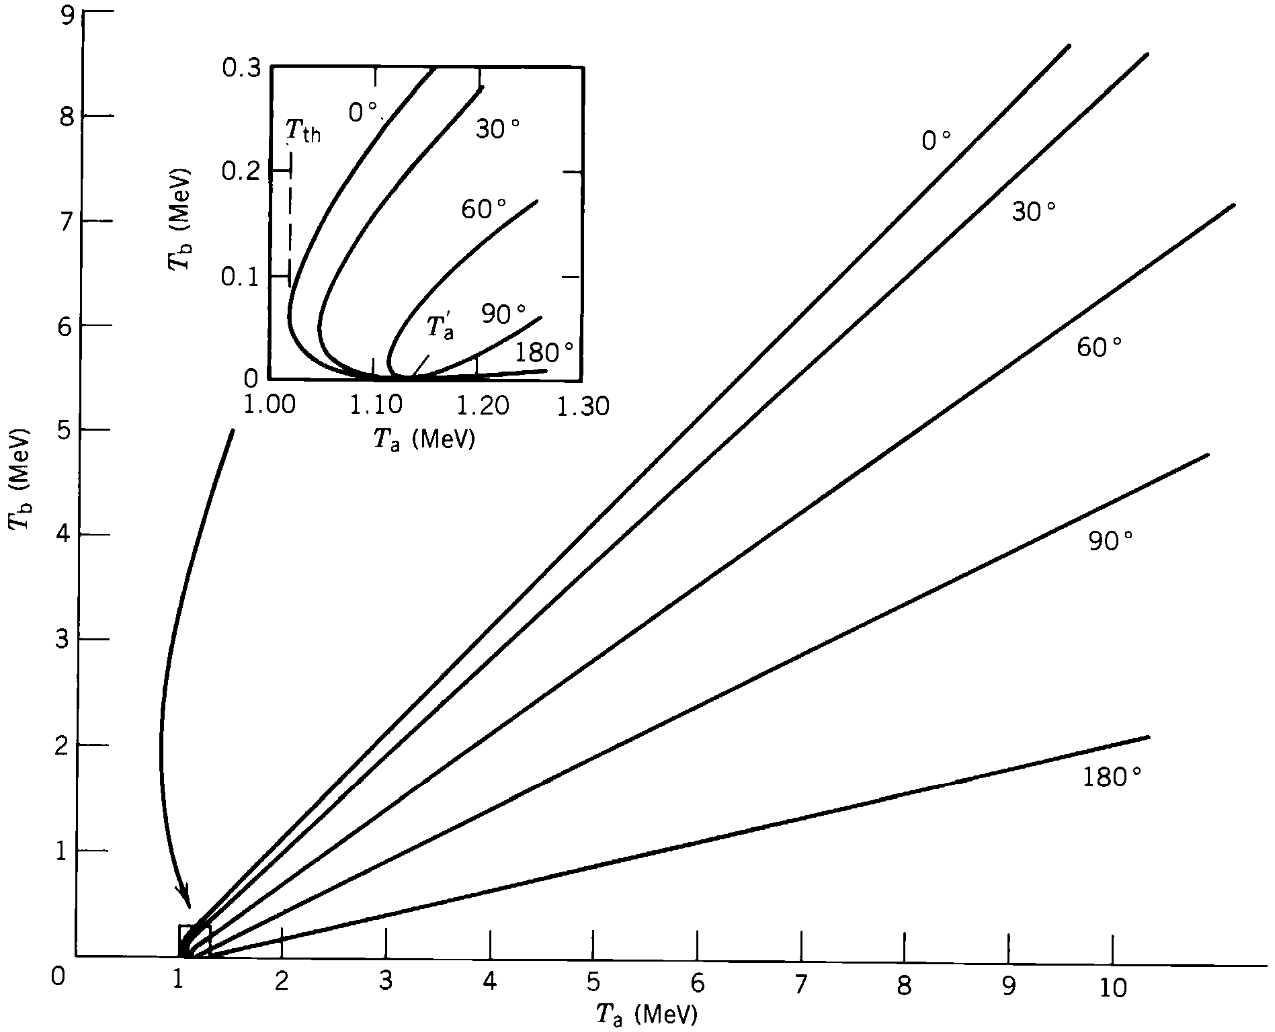
\includegraphics[width=0.70\textwidth]{reac-graph.png}
	\caption{$ T_{\mathrm{b}} $ vs $ T_{\mathrm{b}} $ at various outgoing angles for $ \ch{^3H} \left( p,n \right) \ch{^3He} $.}
	\label{reac-graph}
\end{figure}

\paragraph{Stati eccitati}

È possibile che il nuclide $ \mathrm{Y} $ sia prodotto in uno stato eccitato $ \mathrm{Y}^* $; in tal caso, si vede che il $ Q $-value diminuisce a causa dell'excitation energy $ E_{\text{ex}} $:
\begin{equation}
	Q = Q_0 - E_{\text{ex}}
	\label{eq:6.4}
\end{equation}
dove $ Q_0 $ è relativo alla reazione che produce $ \mathrm{Y} $ nel ground state. È quindi possibile ricostruire lo spettro della specie $ \mathrm{Y} $ calcolando il $ Q $-value a partire da $ T_{\mathrm{a}} $, $ \theta $ (fissati) e $ T_{\mathrm{b}} $ (misurato), il che è possibile invertendo l'Eq. \ref{eq:6.2}:
\begin{equation}
	Q = \left( 1 + \frac{M_{\mathrm{b}}}{M_{\mathrm{Y}}} \right) T_{\mathrm{b}} - \left( 1 - \frac{M_{\mathrm{a}}}{M_{\mathrm{Y}}} \right) T_{\mathrm{a}} - 2 \sqrt{\frac{M_{\mathrm{a}}}{M_{\mathrm{Y}}} \frac{M_{\mathrm{b}}}{M_{\mathrm{Y}}} T_{\mathrm{a}} T_{\mathrm{b}}} \cos \theta
	\label{eq:6.5}
\end{equation}
Solitamente si raggiunge una sufficiente accuratezza utilizzando i numeri atomici al posto delle masse nucleari, specialmente per $ \theta \approx \frac{\pi}{2} $ (si annulla l'ultimo termine).

\paragraph{Cross-section}

Si consideri un projectile beam d'intensità $ \Phi_0 $ (particelle al secondo) diretto su uno strato sottile di nuclei target con spessore $ s $: a causa delle interazioni coi targets, il projectile beam risulta attenuato a seguito del passaggio nello strato sottile, con un'intensità risultante $ \Phi_{\text{f}} $. La frazione di particelle incidenti che reagiscono è funzione della densità numerica di targets $ n_{\text{t}} $ e dalla cross-section $ \sigma $ della reazione:
\begin{equation}
	d\Phi = - \Phi n_{\text{t}} \sigma dx
	\quad \Rightarrow \quad
	\Phi_0 - \Phi_{\text{f}} = \Phi_0 \left( 1 - e^{- n_{\text{t}} \sigma s} \right) \approx \Phi_0 n_{\text{t}} \sigma s
	\label{eq:6.6}
\end{equation}

\paragraph{Trattazione semiclassica}

Classicamente, si può pensare ai nuclidi come sfere rigide che urtano, con vari risultati a seconda del parametro d'impatto $ b $: per $ b \approx R_{\mathrm{X}} $ si ha un urto elastico, per $ b \ll R_{\mathrm{X}} $ ci può essere uno scambio di nucleoni tra i nuclidi, per $ b \approx 0 $ si può arrivare alla formazione di un unico nucleo composto dal nucleo target e da quello incidente.

\section{Reazioni di diffusione e scattering}

Si dicono reazioni di diffusione o di scattering quelle reazioni in cui $ \mathrm{b} = \mathrm{a} $ (o suoi stati eccitati). Si parla di \textit{scattering elastico} per le reazioni $ \mathrm{A} \left( \mathrm{a},\mathrm{a} \right) \mathrm{A} $, di \textit{scattering inelastico} negli altri casi.











